%%%%%%%%%%%%%%%%%%%%%%%%%%%%%%%%%%%%%%%%%%%%%%%%%%%%
% This will help you in writing your homebook
% Remember that the character % is a comment in latex
%
% chapter 1
\chapter{Physical Design}
\label{physical_design}

\section{Introduction}

% Below is shown how you can insert a figure. If you give a label to the figure, you can refer to the figure using \ref{figure_label} as shown above. 
	\begin{figure}[ht]
	\centering
	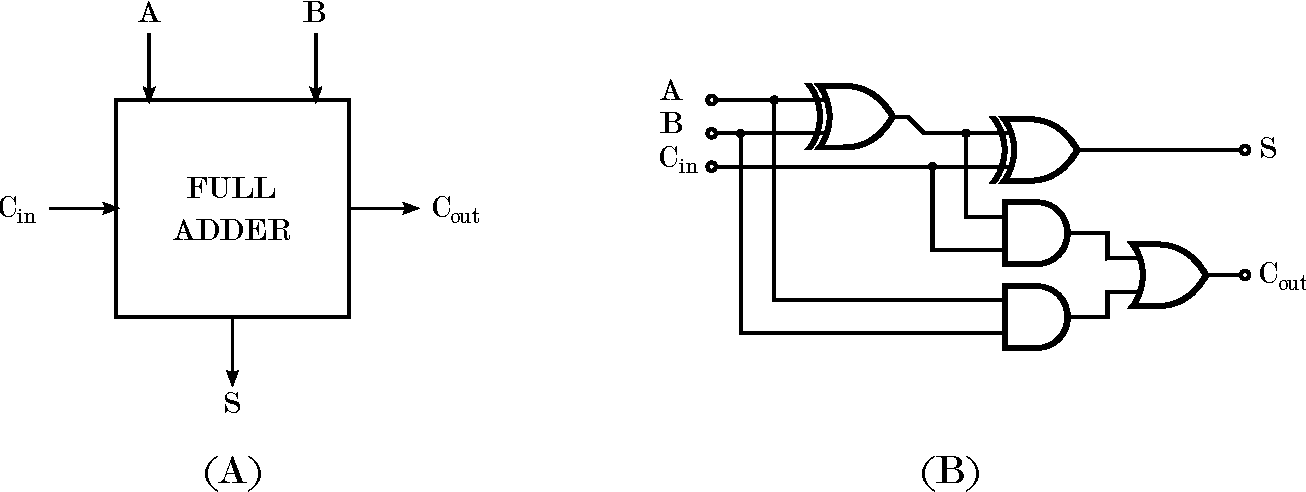
\includegraphics[width=\textwidth]{chapters/figures/fa} 
	\caption{(A) Schematic symbol of a 1-bit full adder. A and B are the operands, Cin is the carry-in while Cout and S are the carry-out and the sum, respectively. (B) Logic diagram of the 1-bit full adder.}
	\label{fig:fa}  % here is the figure label
	\end{figure}

This is the final step, in which the layout of our DLX design can be generated, using the \textbf{Innovus} tool, provided by Cadence.
The entire procedure is composed of various steps, from Floorplanning to Cell Placing and signal Routing.

To start creating the floorplan, Innovus needs a verilog post-synthesis netlist, a \textit{.lef} file that has references to the library of cells and other data which is
provided in the project files. In this step the area dedicated to the chip core is computed, along with the power supply rings around it.
%% put figure
Next, the power rings for \textit{Vdd} and \textit{GND} are inserted in the model and on the layout corner, the vias to connect the metal layer are placed as well. To avoid congestion, M9 and M10 metals are chosen for the rings.





















